%===================================== CHAP 5 =================================

\chapter{Architecture and implementation, Not finished}

This chapter explains the processes and solutions made in the design phase of the solution. It also explains the actual implementation of the system.

\section{User interface}

One of the initial requirements from the customer, was to have a graphical user interface. It was supposed to display relevant data and allow the administrator to moderate topics. After an initial consideration, Spring MVC was chosen to be the most suitable. The framework deploys the standard MVC pattern in Java. The framework is designed around a dispatcherServlet. This central component is responsible for receiving the incoming HTTP requests, and passing the requests onto the correct controller. The methods used to handle the requests are notated with the @Controller and @Restcontroller notations. The controller methods are responsible for returning data to the dispatcherServlet, which then writes the web response objects.  [!!!!!!!!!IFFY; VET IKKE HELT OM STEMMER, ADDMORELATER!!!!!!!!!]

The interface contains five panes. The main pane and the stats pane contain information about the broker. The main pane is meant to give a general overview of of the current operating environment, as well as the system status. The stats pane contain information about the general usage, as well as requests over the different protocols. The logs pane contains runtime logs for debugging purposes. Finally, the topics pane and config pane allows you to view, remove and map topics to each other.

\section{Broker architecture}

\section{Implementation}

\subsection{WSN}

Here be information about how WSN was implemented, as well as how it works

\subsection{AMQP}

Here be information about how AMQP was implemented, as well as how it works

\clearpage

\section{Message workflow}

\begin{center}
  \begin{figure}[ht!]
    \makebox[\textwidth]{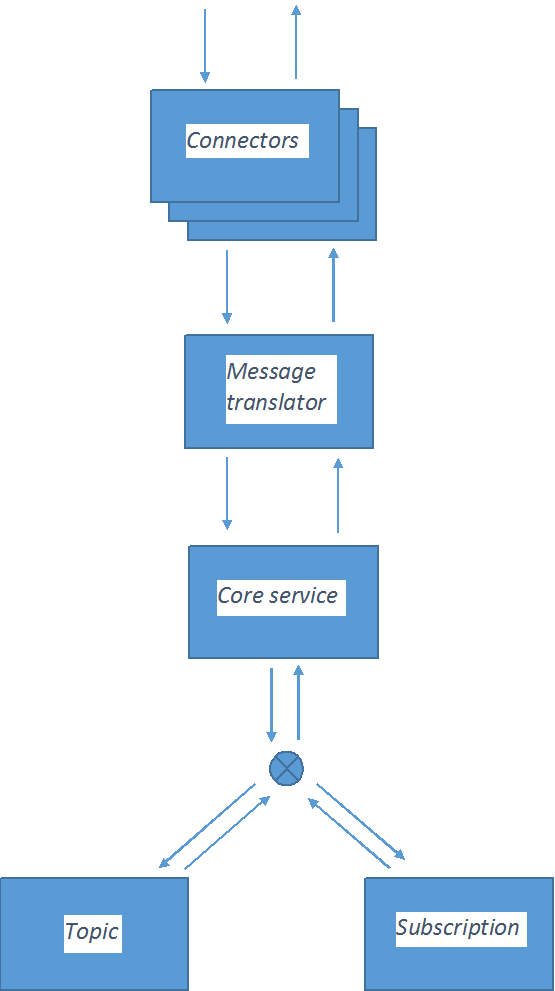
\includegraphics[scale=0.3]{fig/MessageWorkflow.png}}
    \caption{Message workflow}
    \label{fig:Message workflow}
  \end{figure}
\end{center}

\clearpage